%% using aastex version 6.2
\documentclass[twocolumn, dvipdfmx]{aastex62}
\usepackage{CJK}
\usepackage{textcomp}
\usepackage{graphicx}
\usepackage{here}
\usepackage{hhline}
\usepackage{longtable}

\def\hoge<#1>{\langle #1 \rangle}
\newcommand\aastex{AAS\TeX}
\newcommand\latex{La\TeX}

\received{\today}
\revised{\today}
\accepted{\today}
\submitjournal{ApJ}

\shortauthors{Goda \& Matsuo}

\begin{document}
\begin{CJK*}{UTF8}{min}

\title{Title}

\author{Shohei Goda}
\affil{\rm Department of Earth and Space Science, Graduate School of Science, Osaka University, 1-1, Machikaneyamacho, Toyonaka, Osaka 560-0043, Japan}

\author{Taro Matsuo}
\affiliation{\rm Department of Earth and Space Science, Graduate School of Science, Osaka University, 1-1, Machikaneyamacho, Toyonaka, Osaka 560-0043, Japan}


\begin{abstract}

太陽系外惑星の性質を統計的に理解することにより、惑星系の形成過程を明らかにすることが期待される。惑星系の重要なパラメータとして主星の金属量と惑星の質量がある。主星の金属量は、原始惑星系円盤における惑星の材料物質である微惑星の量を反映すると考えられている。金属量の高い主星の周りでは、コア集積により円盤ガスの散逸前までにコアの臨界質量に達するため巨大ガス惑星が形成されやすく、惑星の検出確率が主星の金属量と正の相関を持つ観測結果を説明できると考えられている。また、ボトムアップから惑星が成長するため、惑星質量が連続的に分布する傾向にあると予想される。他方、重力不安定による惑星形成は、原始惑星系円盤の質量と温度に依存するため、主星の金属量には強く依存しないと考えられる。また、ボトムアップからの形成でないため、惑星の質量分布も低質量から連続的に分布しないことが予想される。以上を踏まえて、私たちは主星の金属量の高い領域と低い領域における惑星分布を統計的に明らかにし、惑星形成過程を理解することを試みる。ここでは惑星検出の選択効果を考慮した上で議論を進めるため、金属量の高い(あるいは低い)惑星サンプルに対して金属量の低い(あるいは高い)惑星検出の選択効果を掛け合わせて惑星分布が選択効果に依存しないようにデータセットを作成した。そのデータセットに対して混合正規分布モデルで分類を行なった結果、金属量の違いに関わらず3木星質量と15木星質量付近を境に異なる集合として分布することがわかった。また、金属量の低い領域における惑星質量分布が低質量からの連続的なものではなく、高い領域のものと大きく異なることが分かった。さらに惑星の軌道長半径と軌道離心率に関しても領域ごとの違いが見られた。本論では、統計的解析の過程について述べ、解析から得られた惑星分布の結果に対して惑星の形成過程、およびを考察する。


\end{abstract}

\vspace{1cm}

\keywords{methods: data analysis -- planets and satellites: terrestrial planets}


\section{Introduction} \label{sec:introduction}

数十年前に太陽系内の惑星形成についての議論が発達し\citep{1985Arizona}、木星サイズの惑星に対して2つの形成理論が提案された。一つはコア集積であり\citep{1974Icar...22..416P, 1980PThPh..64..544M, 1996Icar..124...62P}、もう一つは円盤不安定である\citep{1951PNAS...37....1K, 1997Sci...276.1836B, 2002Sci...298.1756M}。理論上、その二つの惑星形成過程は円盤の金属量に異なる依存性を示す。ここで金属量とは、水素原子に対する金属の数密度の比を表す。コア集積モデルの場合、コアの種となる部分が成長する必要があるため、この成長を促進する金属量の多い領域に対して起こりやすい\citep{2004ApJ...616..567I, 2012A&A...541A..97M}。一方、円盤不安定による惑星形成の場合、円盤の冷却時間を長くする必要があるため、より厚い円盤を持つことが重要である。つまり厚い円盤を形成しやすいとされる、金属量の少ない領域に対して起こりやすい\citep{2006ApJ...636L.149C, 2007Arizona}。ただし、観測された惑星系において、円盤の金属量と円盤不安定には相関がないと主張する論文\citep{2002ApJ...567L.149B}や、わずかながら正の相関があると提唱する論文\citep{2007ApJ...661L..77M}もある。木星型惑星のエンベロープは太陽のそれと比べて重元素で構成されているため\citep{2003NewAR..47....1Y}、コア集積モデルは木星型惑星に対して標準な形成過程として広く受け入れられている。

1995年に標準星の周りを周回している惑星が初めて発見されて以来\citep{1995Natur.378..355M}、広視野での視線速度法観測によって、太陽系外の巨大ガス惑星は金属量が豊富な主星の周りに存在しやすく\citep{2003A&A...398..363S, 2005ApJ...622.1102F}、小さい惑星を持つ惑星系の金属量は、巨大ガス惑星を持つ惑星系の金属量に比べて少ないことが明らかにされた\citep{2011arXiv1109.2497M, 2015AJ....149...14W}。中心星とその周りにある原始惑星系円盤は、同一の分子雲で構成されているため、ほとんどの巨大ガス惑星はコア集積を経由して形成されたと思われる\citep{2004ApJ...616..567I, 2012A&A...541A..97M}。直接撮像によって発見された惑星の中には、コア集積で形成された惑星が惑星移動や惑星間による散乱によって広がったと説明するよりも、円盤の重力不安定によって形成されたと説明した方が納得のいく惑星も存在する\citep{2009ApJ...707...79D}。一方、最近の論文によると10 au以遠の大質量コアはペブル集積によって形成される可能性があるため\citep{2010A&A...520A..43O, 2012A&A...544A..32L}、直接撮像された惑星はペブル集積モデルによって説明することもできる。こうしてこれらの惑星形成過程を用いることにより、幅広い多様な惑星系を説明することができる。

今まで議論されてきた惑星形成過程は観測データの分布より考察されている。これは観測データによる分布が真の分布に近いことを仮定した場合を想定している。しかし、得られたデータの中には望遠鏡の観測精度や、目標天体に対する観測期間が十分でないデータも含まれており、その精度は金属量の違いによって偏りが生じている。精度の悪い観測や、短い観測期間によって検出可能な惑星には制限がついてしまう。つまり、これまでに発見されてきた惑星から得た分布には、選択効果によって欠損している領域の存在可能性がある。

本論では、この選択効果による影響が実際に惑星の分布にどの程度影響しているのかを議論し、その結果を元に巨大ガス惑星の形成過程について述べる。第2章では本論で採用した惑星サンプルの説明、および選択効果を考慮した場合の惑星分布の分類の手法について述べる。第3章では分類した領域ごとの軌道長半径と軌道離心率の分布を調べ、そこから言える惑星形成過程や進化について議論する。


\section{Method} \label{sec:method}

この章では惑星分布を確かめるためのシミュレーションの準備とその方法について述べる。


\subsection{Preparing data} \label{subsec:prepare}

視線速度法で観測された惑星のリストと、その惑星による主星の視線速度、惑星の軌道周期、および軌道離心率の値をexoplanet.euから取り出した。一方、主星の質量と金属量をSweet-catカタログから取り出し、\cite{2008ApJ...677.1324T}に掲載されている式を用いて惑星質量の下限値を求めた。また、取り出した軌道周期と主星質量より、惑星の軌道長半径を求めた。主星の質量と金属量が不足しているデータに関しては、Casagrandeカタログ\citep{2011A&A...530A.138C}とPdovaカタログ\citep{2011MNRAS.416..727C}、およびBastiカタログ(参考文献が見つからない)から取り出し、Sweet-catカタログとの相関を調べ、線形変換を行った。また、選択効果の指標となる各惑星系に対する観測精度と観測期間に関してはexoplanets.orgから取り出した。観測期間と主星の質量によりその惑星系で見つけられる惑星の最大軌道長半径を求めることができ、その最大軌道長半径と主星質量、および観測精度により観測可能な最小の惑星質量を求めることができる。その他欠損しているデータに関しては参考文献を参照した。結果、これらの惑星のうち惑星質量が0.1木星質量以上のものを対象にした場合、520個の惑星系と623個の惑星をサンプルとして取り出せた。ここで0.1木星質量で区切る理由は、この領域における観測された惑星サンプル数が過疎化しており、本論で議論する際の分類に影響を与えるためである(参考文献があれば入れる)。


\subsection{Examination of selection bias} \label{subsec:bias}

異なる金属量領域の選択効果による影響を調べるため、二つの領域における惑星質量分布が最も異なるように金属量の境界値を求める。ここで検定としてアンダーソンダーリン検定(AD検定)を使用し、各境界値の場合のp値を比較した。ここで、異なる金属量領域の選択効果を排除するために、金属量の高い(低い)領域の惑星データに金属量の低い(高い)領域の選択効果をかけた。惑星パラメータの値を誤差を考慮してランダムに取り出し、選択効果もランダムにかけることで計算の偏りをなくし、最適な境界値が収束するのに十分な回数でシミュレーションを行った。その結果、最適な金属量の境界値は-0.09 [Fe/H]となり、その時のp値は$5.6\times10^{-5}$であった。この値は二つの分布が異なるものであることを証明するのに十分な値であり、選択効果を考慮した結果、観測された二つの金属量領域における惑星質量分布は異なるものであることが言えた。


\subsection{Classification of planetary distribution with Gaussian Mixture Model} \label{subsec:classification}

最適化された金属量の境界値を用いて惑星サンプルを二つの領域にわけ、それぞれの惑星分布を分類器を用いて分類していく。今回使用した分類器は正規混合モデルであり、これは各データ点がある値を中心に正規分布をしていることを仮定し、クラスターの数に応じて分類するものである。それぞれのクラスター数におけるモデルをBayesian Information Criterion (BIC)を用いて評価し、最適なクラスター数を求めた結果、高金属量領域、低金属量領域共にクラスター数が3の時が最適となり、その時のBICの点数はそれぞれ2644と1197であった。図\ref{fig:a_Mp}の上図は最適なクラスター数の時に惑星分布を分類した結果であり、黒の点線は3つの領域を隔てる惑星質量の境界線である。高金属量領域の場合、境界線は$2.8 M_J$と$11.5 M_J$に引かれ、低金属量領域の場合は$3.5 M_J$と$20.0 M_J$に引かれた。

\begin{figure}[t]
\begin{center}
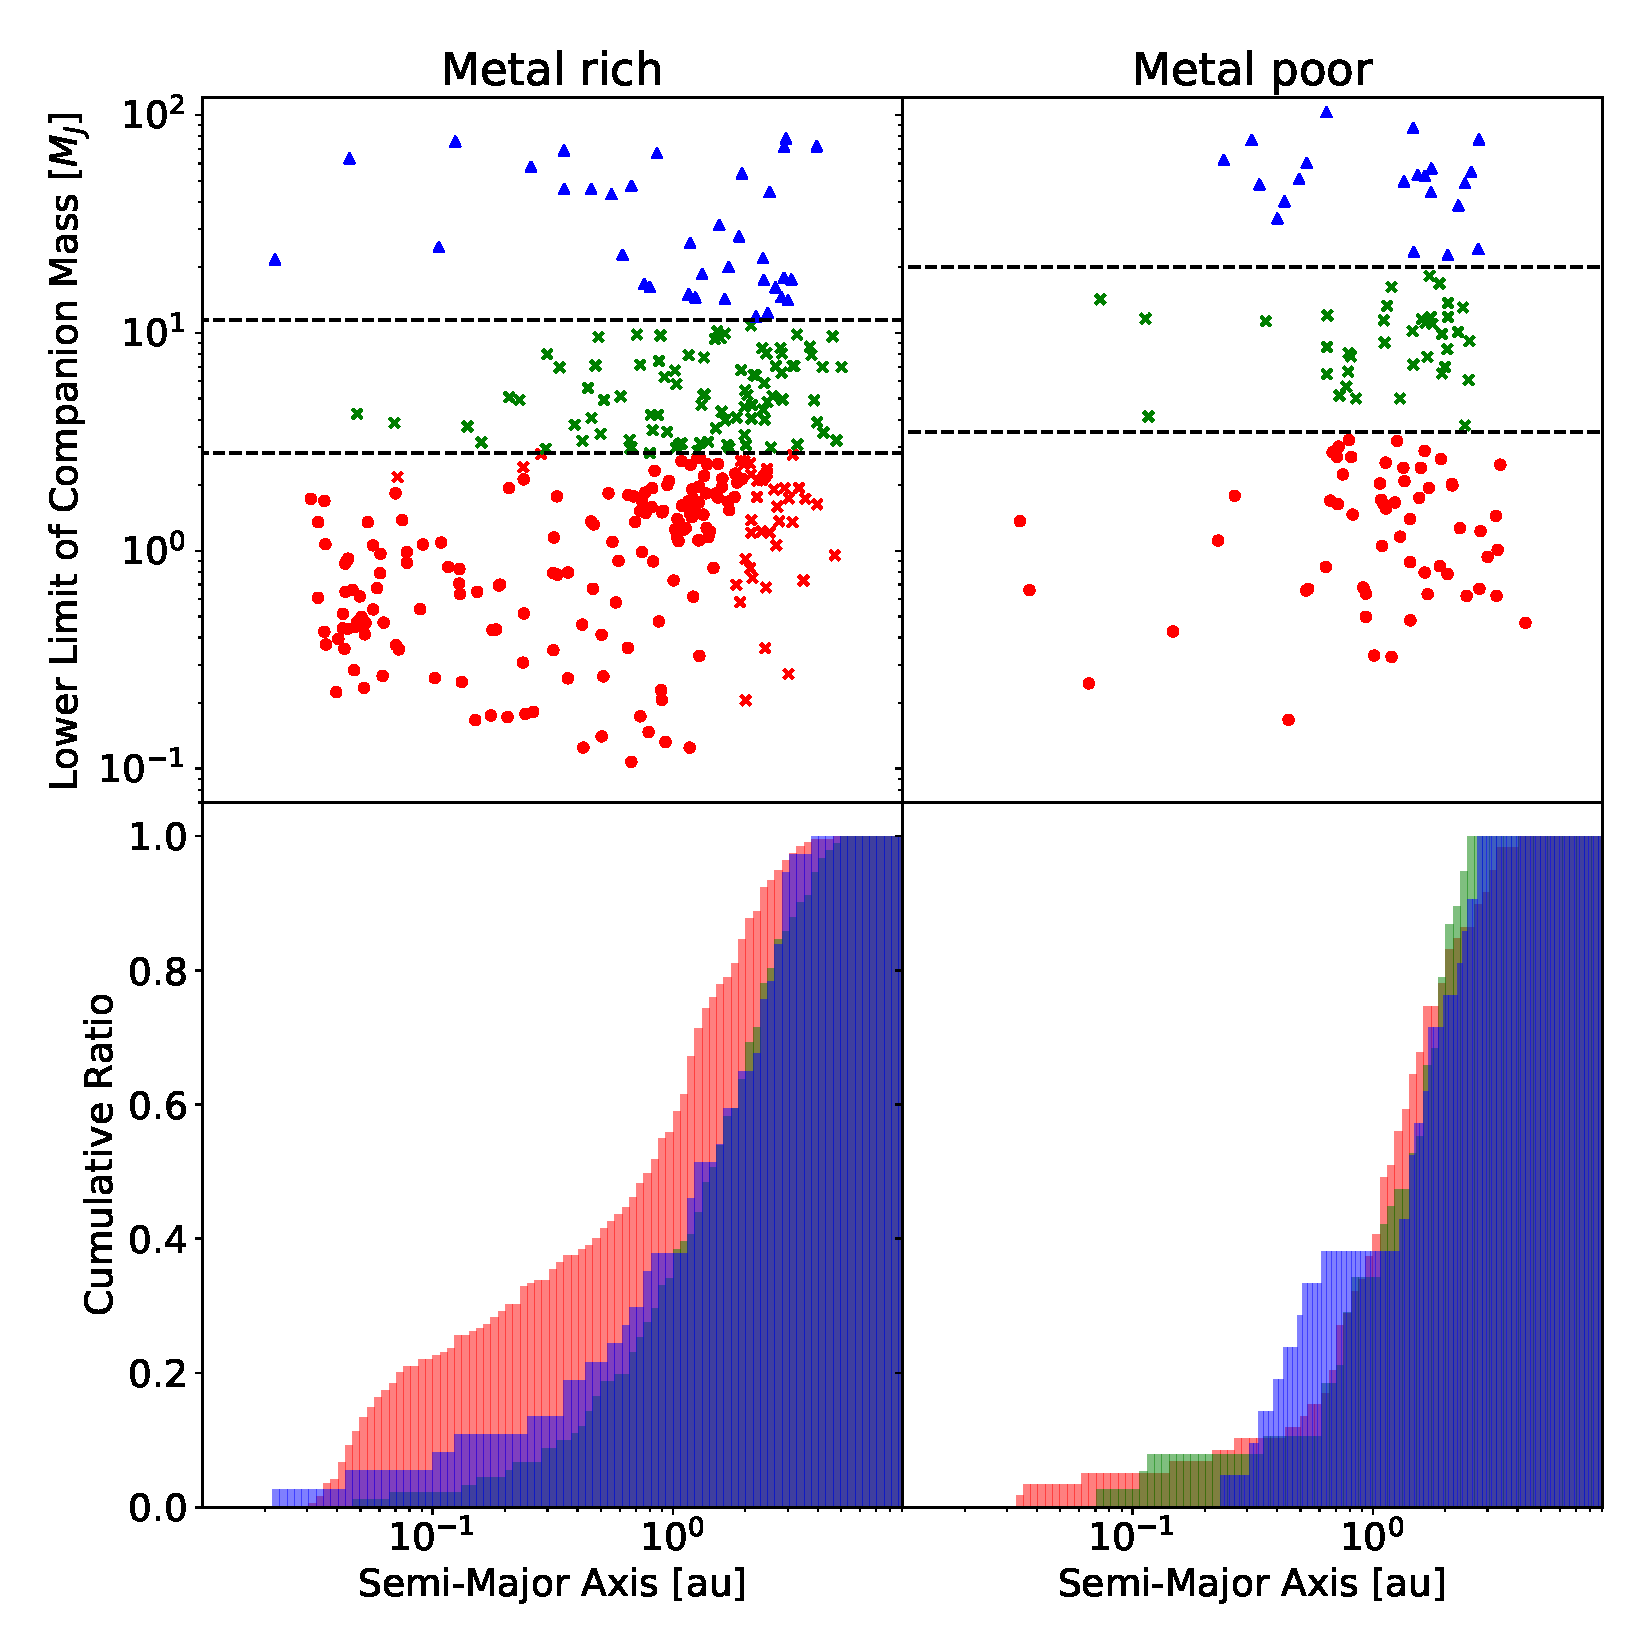
\includegraphics[width=9cm]{../../Figure/a_Mp_merge.pdf}
\caption{惑星の軌道長半径と惑星質量の散布図(上図)と軌道長半径の累積分布(下図)。上図の記号は正規混合モデルにより分類したラベルの違いを表し、そのラベルの分布より惑星質量の境界値を定め、破線でその境界線を引いている。また、境界線で分けた3つの領域を異なる色でプロットしている。これらの色は下図の色と一致している。\label{fig:a_Mp}}
\end{center}
\end{figure}


\section{Results} \label{sec:results}

正規混合モデルで分類した結果を元に得られた惑星質量の境界線より、高金属量領域と低金属量領域における惑星分布はそれぞれ3つずつ得られる。この章では、各々のクラスターにおいて惑星の軌道長半径分布と軌道離心率分布についての考察を行う。


\subsection{Semi-major axis distribution} \label{subsec:axis}

図\ref{fig:a_Mp}の下図は惑星の軌道長半径の累積分布である。惑星質量の小さい領域から赤、緑、青色で示している。金属量が豊富な領域を見ると、低質量領域と中・高質量領域の分布に違いがあることがわかる。これらを比較した場合、p値はそれぞれ$1.0\times10^{-5}$と$3.2\times10^{-3}$であった。これは分布の様子が異なることを十分に説明できる値である。また、金属量の乏しい系における低質量領域とのp値は$1.2\times10^{-3}$であり、金属量の違いによっても異なる分布を説明することができる。これは(思案中)を意味する。


\subsection{Eccentricity distribution} \label{subsec:eccentricity}

図\ref{fig:e_Mp}の上図は最適な金属量の境界値により惑星の分類した軌道離心率と惑星質量の散布図である。下図は軌道離心率の累積分布である。それぞれの色は図\ref{fig:a_Mp}と同様の意味を表す。低金属量側を見ると、高質量領域は他の領域と比べ離心率分布が一様であることがわかる。実際にp値をとると、高質量領域と低・中質量領域を比べた場合、それぞれ$2.3\times10^{-3}$と$1.1\times10^{-2}$であった。これは高質量領域の惑星が(思案中)であることを示唆する。一方、高金属量側の分布では、中・高質量領域の惑星が一様に分布していることがわかる。低質量領域と中・高質量領域のp値をとると、それぞれ$1.6\times10^{-5}$と$4.4\times10^{-4}$であった。これは金属量の高い惑星系において惑星同士の重力散乱が中質量の惑星で起きていることを示唆する。なぜならコア集積モデルを考えた場合、金属量の豊富な領域でより多くのコアが形成され、一つの系に複数の巨大ガス惑星が形成される可能性が高くなるからである。

\begin{figure}[H]
\begin{center}
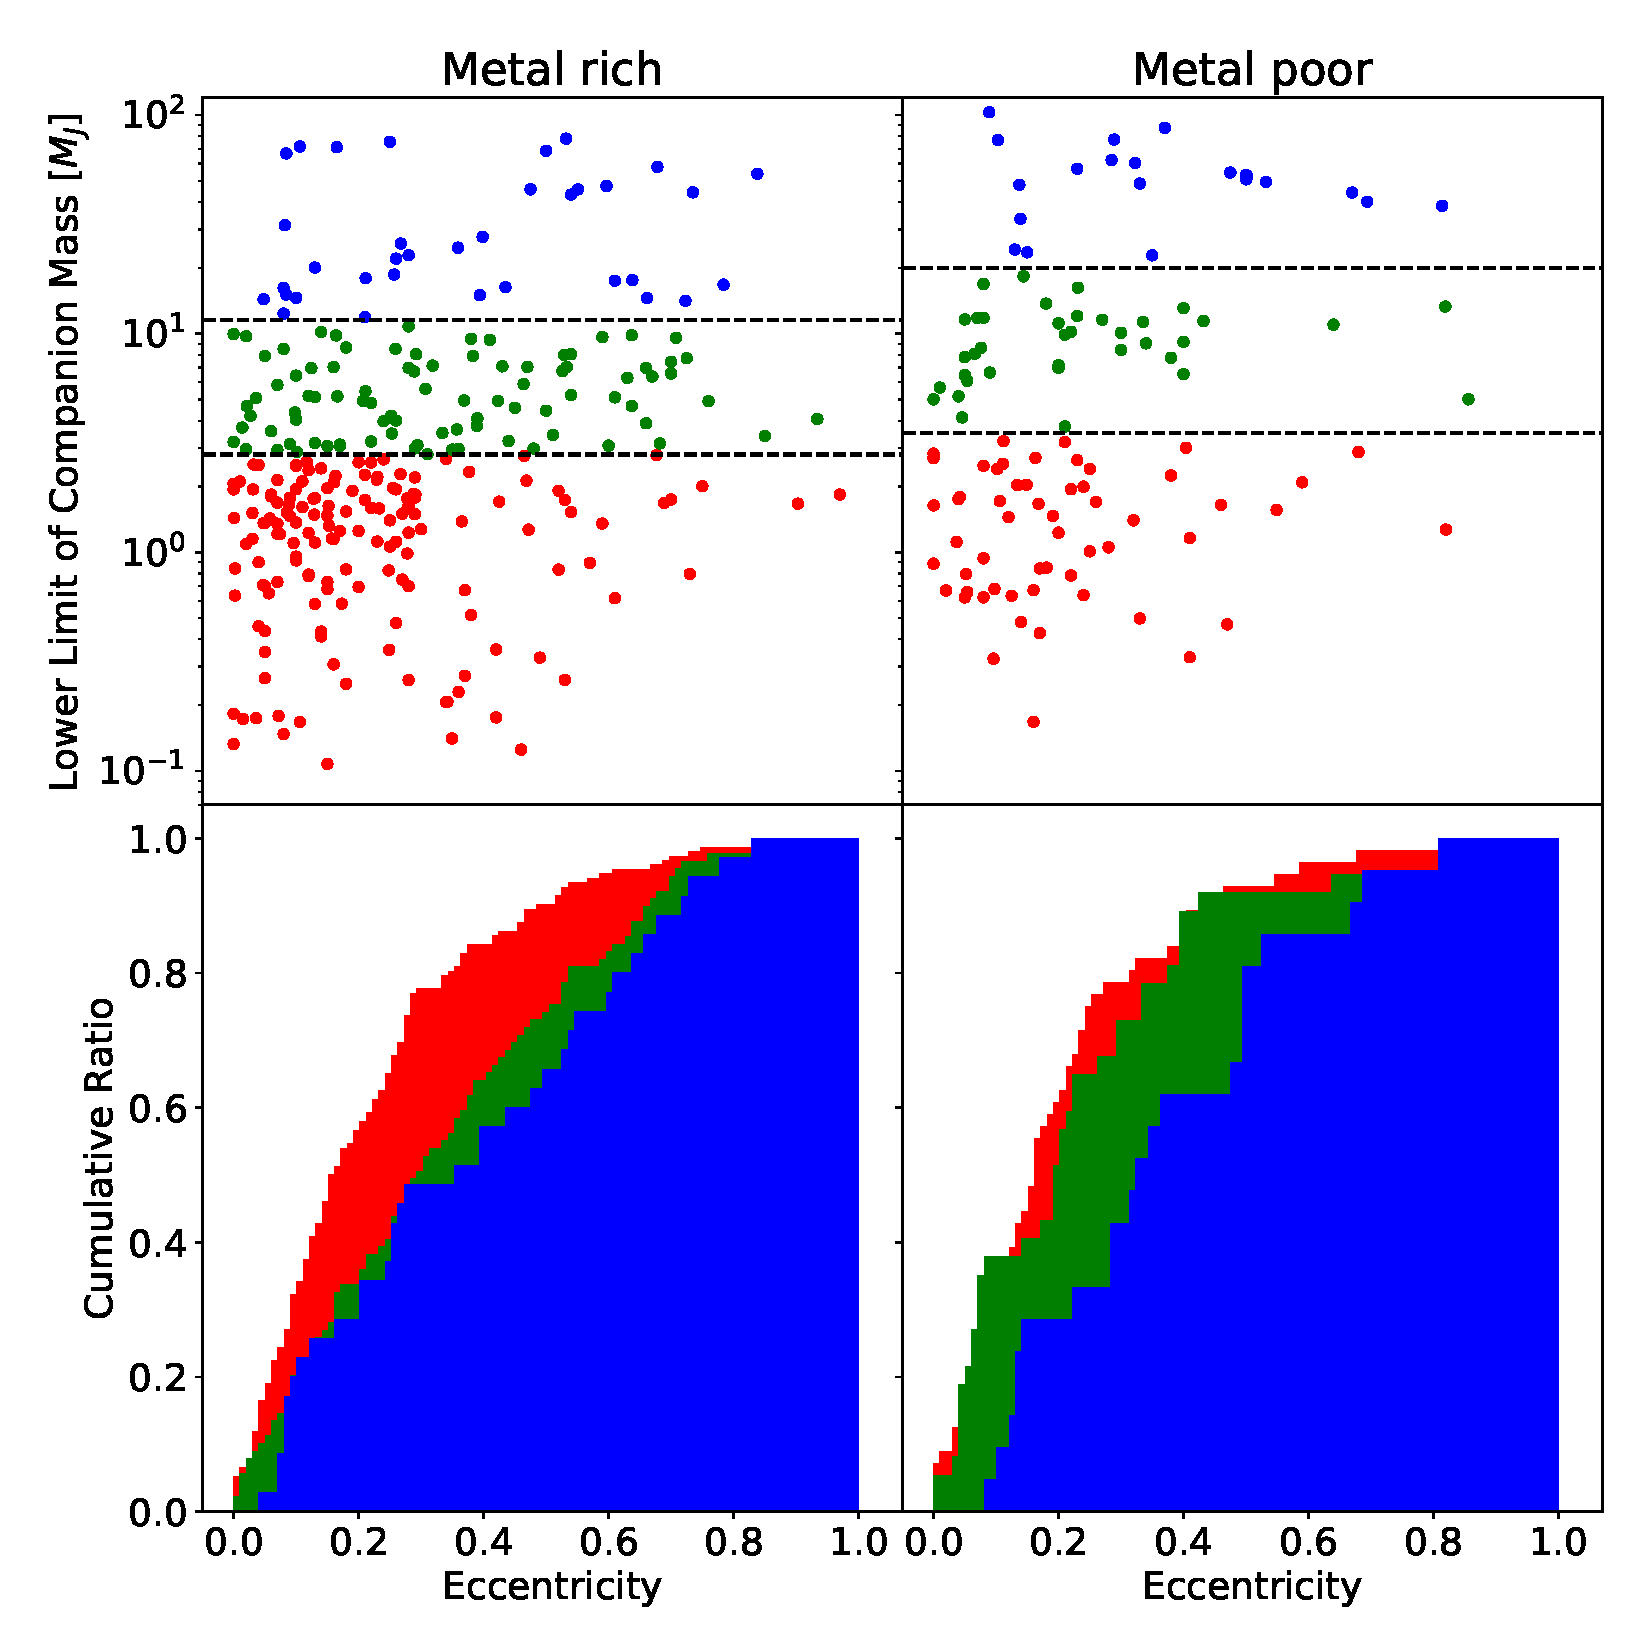
\includegraphics[width=9cm]{../../Figure/e_Mp_merge.pdf}
\caption{惑星の軌道離心率と惑星質量の散布図(上図)と軌道離心率の累積分布(下図)。図\ref{fig:a_Mp}の上図と同様、惑星質量の境界線を元に色分けをしており、下図の色と対応させている。\label{fig:e_Mp}}
\end{center}
\end{figure}


\acknowledgments


\vspace{5mm}


\begin{thebibliography}{}

\bibitem[Boss(1997)]{1997Sci...276.1836B} Boss, A.~P.\ 1997, Science, 276, 1836
\bibitem[Boss(2002)]{2002ApJ...567L.149B} Boss, A.~P.\ 2002, \apjl, 567, L149
\bibitem[Cai et al.(2006)]{2006ApJ...636L.149C} Cai, K., Durisen, R.~H., Michael, S., et al.\ 2006, \apjl, 636, L149
\bibitem[Calvi et al.(2011)]{2011MNRAS.416..727C} Calvi, R., Poggianti, B.~M., \& Vulcani, B.\ 2011, \mnras, 416, 727
\bibitem[Casagrande et al.(2011)]{2011A&A...530A.138C} Casagrande, L., Sch{\"o}nrich, R., Asplund, M., et al.\ 2011, \aap, 530, A138
\bibitem[Dodson-Robinson et al.(2009)]{2009ApJ...707...79D} Dodson-Robinson, S.~E., Veras, D., Ford, E.~B., \& Beichman, C.~A.\ 2009, \apj, 707, 79
\bibitem[Durisen et al.(2007)]{2007Arizona} Durisen, R. H., Reipurth, V. Jewitt, Keil, K., et al.\ 2007, Univ. of Arizona Press, Tucson 951, 607-622
\bibitem[Fischer \& Valenti(2005)]{2005ApJ...622.1102F} Fischer, D.~A., \& Valenti, J.\ 2005, \apj, 622, 1102
\bibitem[Hayashi\&Nakagawa(1985)]{1985Arizona} Hayahi, C., Nakazawa, K., \& Nakagawa, Y.\ 1985, Formation of the solar system. Protostars and Planets II. Tucson AZ, University of Arizona Press 1100-1153
\bibitem[Ida \& Lin(2004)]{2004ApJ...616..567I} Ida, S., \& Lin, D.~N.~C.\ 2004, \apj, 616, 567
\bibitem[Kuiper(1951)]{1951PNAS...37....1K} Kuiper, G.~P.\ 1951, Proceedings of the National Academy of Science, 37, 1
\bibitem[Lambrechts \& Johansen(2012)]{2012A&A...544A..32L} Lambrechts, M., \& Johansen, A.\ 2012, \aap, 544, A32
\bibitem[Mayor \& Queloz(1995)]{1995Natur.378..355M} Mayor, M., \& Queloz, D.\ 1995, \nat, 378, 355
\bibitem[Mayer et al.(2002)]{2002Sci...298.1756M} Mayer, L., Quinn, T., Wadsley, J., \& Stadel, J.\ 2002, Science, 298, 1756
\bibitem[Mayer et al.(2007)]{2007ApJ...661L..77M} Mayer, L., Lufkin, G., Quinn, T., \& Wadsley, J.\ 2007, \apjl, 661, L77
\bibitem[Mayor et al.(2011)]{2011arXiv1109.2497M} Mayor, M., Marmier, M., Lovis, C., et al.\ 2011, arXiv:1109.2497
\bibitem[Mizuno(1980)]{1980PThPh..64..544M} Mizuno, H.\ 1980, Progress of Theoretical Physics, 64, 544
\bibitem[Mordasini et al.(2012)]{2012A&A...541A..97M} Mordasini, C., Alibert, Y., Benz, W., Klahr, H., \& Henning, T.\ 2012, \aap, 541, A97
\bibitem[Ormel \& Klahr(2010)]{2010A&A...520A..43O} Ormel, C.~W., \& Klahr, H.~H.\ 2010, \aap, 520, A43
\bibitem[Perri \& Cameron(1974)]{1974Icar...22..416P} Perri, F., \& Cameron, A.~G.~W.\ 1974, \icarus, 22, 416
\bibitem[Pollack et al.(1996)]{1996Icar..124...62P} Pollack, J.~B., Hubickyj, O., Bodenheimer, P., et al.\ 1996, \icarus, 124, 62
\bibitem[Santos et al.(2003)]{2003A&A...398..363S} Santos, N.~C., Israelian, G., Mayor, M., Rebolo, R., \& Udry, S.\ 2003, \aap, 398, 363
\bibitem[Torres et al.(2008)]{2008ApJ...677.1324T} Torres, G., Winn, J.~N., \& Holman, M.~J.\ 2008, \apj, 677, 1324
\bibitem[Wang \& Fischer(2015)]{2015AJ....149...14W} Wang, J., \& Fischer, D.~A.\ 2015, \aj, 149, 14
\bibitem[Young(2003)]{2003NewAR..47....1Y} Young, R.~E.\ 2003, \nar, 47, 1

\end{thebibliography}

\appendix

\end{CJK*}
\end{document}
